\documentclass[12pt,a4paper]{report}

% --- PACKAGES ---
\usepackage[utf8]{inputenc}
\usepackage{mathptmx} % Font Times New Roman
\usepackage{graphicx} % Untuk memasukkan gambar/logo
\usepackage{geometry} % Mengatur margin
\geometry{
    top=3cm, 
    bottom=3cm, 
    left=4cm, 
    right=3cm
}
\usepackage{setspace} % Mengatur spasi antar baris
\usepackage{titlesec} % Mengatur format judul bab dan sub-bab
\usepackage{indentfirst} % Indentasi paragraf pertama
\usepackage[labelfont=bf, labelsep=space]{caption}
\usepackage{longtable} % Untuk tabel panjang yang memotong halaman
\usepackage{booktabs} % Untuk garis tabel yang lebih rapi
\usepackage{cite} % Untuk sitasi bergaya IEEE\\)
\usepackage{multirow}
\usepackage{changepage}
\usepackage{microtype}
\usepackage[indonesian]{babel}
\usepackage{array}          % Untuk mengatur format teks dalam kolom tabel
\usepackage[table]{xcolor}  % Untuk memberikan warna pada sel tabel (cellcolor)
\definecolor{lightgreen}{RGB}{144, 238, 144}
\usepackage{float}          % Untuk menggunakan opsi posisi [H] (paksa diam di tempat)
\usepackage{hyperref}
\hypersetup{
    colorlinks=true,   % Mengaktifkan warna pada link (bukan kotak jelek)
    linkcolor=black,   % Warna link internal (daftar isi, gambar, tabel)
    citecolor=blue,    % Warna sitasi ke daftar pustaka (misal: [1], [2])
    urlcolor=blue      % Warna link website/URL
}

% --- FORMATTING BAB & SUB-BAB ---
\renewcommand{\chaptername}{BAB}
\renewcommand{\thechapter}{\Roman{chapter}} 
\renewcommand{\contentsname}{DAFTAR ISI}
\renewcommand{\listfigurename}{DAFTAR GAMBAR}
\renewcommand{\listtablename}{DAFTAR TABEL}
\titleformat{\chapter}[display]
  {\normalfont\large\bfseries\centering}{BAB\ \thechapter}{5pt}{\large}
\titlespacing*{\chapter}{0pt}{-20pt}{20pt}

% Format Sub-bab (A, B, C, ...)
\renewcommand{\thesection}{\Alph{section}.}
\titleformat{\section}
  {\normalfont\normalsize\bfseries}{\thesection}{1em}{}

% Format Sub-sub-bab (1, 2, 3, ...)
\renewcommand{\thesubsection}{\arabic{subsection}.}
\titleformat{\subsection}
  {\normalfont\normalsize\bfseries}{\thesubsection}{1em}{}

\renewcommand{\thesubsubsection}{\alph{subsubsection}.}

% Memaksa penomoran Gambar, Tabel, dan Persamaan memakai Angka Arab murni (e.g., 3.1)
\makeatletter
\renewcommand{\thefigure}{\the\value{chapter}.\arabic{figure}}
\renewcommand{\thetable}{\the\value{chapter}.\arabic{table}}
\renewcommand{\theequation}{\the\value{chapter}.\arabic{equation}}
\makeatother

\renewcommand{\chapterautorefname}{Bab}
\renewcommand{\figureautorefname}{Gambar}
\renewcommand{\tableautorefname}{Tabel}
% --- INFORMASI DOKUMEN ---
\newcommand{\judulProposal}{ANALISIS DAN OPTIMASI SISTEM DETEKSI KERETAKAN PIPA BERBASIS GAMMA COMPTON \textit{BACKSCATTERING} DENGAN GEANT4 DAN TOMOGRAPHY}
\newcommand{\namaMahasiswa}{ARDIANSAH NUR ROHMAN}
\newcommand{\nimMahasiswa}{230322607922}
\newcommand{\namaKBK}{FISIKA KOMPUTASIONAL DAN TEORITIK}
\newcommand{\dosenSatu}{Dr. Hafizh Prihtiadi, S. Si., M. Si.}
\newcommand{\nipSatu}{198804082024061001}
\newcommand{\dosenDua}{Dr. Hari Wisodo, S. Si., M. Si.}
\newcommand{\nipDua}{197307241998031001}
\newcommand{\bulanTahun}{AGUSTUS 2026}

\begin{document}
\onehalfspacing % Set spasi 1.5 untuk teks utama

% ==========================================
% HALAMAN SAMPUL
% ==========================================
\begin{titlepage}
    \centering
    {\large \textbf{PROPOSAL SKRIPSI}}\\[1cm]
    
    \begin{spacing}{1.5}
        {\fontsize{14pt}{21pt} \bfseries \judulProposal}
    \end{spacing}

    \vspace{2cm}

    % Pastikan ada file logo_um.png di folder yang sama
    
\includegraphics[width=3cm]{figs/images.png}\\[1.5cm]
    
    \textbf{DISUSUN OLEH}\\
    \textbf{\namaMahasiswa}\\
    \textbf{NIM \nimMahasiswa}\\
    \vspace{1.5cm}
    \textbf{KBK \namaKBK}\\[1.5cm]
    
    \textbf{DOSEN PEMBIMBING}\\
    \dosenSatu \hspace{0.5cm} NIP \nipSatu \\
    \dosenDua \hspace{0.5cm} NIP \nipDua \\[1.5cm]
    
    \vfill
    
    \textbf{UNIVERSITAS NEGERI MALANG}\\
    \textbf{FAKULTAS MATEMATIKA DAN ILMU PENGETAHUAN ALAM}\\
    \textbf{PROGRAM STUDI FISIKA}\\
    \textbf{\bulanTahun}
    \end{titlepage}
    % --- MULAI PENOMORAN ROMAWI ---
    \pagenumbering{roman}
    \setcounter{page}{2} % Set ke halaman ii (karena halaman i adalah sampul)

    % ==========================================
    % LEMBAR PERSETUJUAN
    % ==========================================
    \newpage
    \chapter*{LEMBAR PERSETUJUAN PEMBIMBING PROPOSAL SKRIPSI}
    \addcontentsline{toc}{chapter}{LEMBAR PERSETUJUAN}

    \noindent Proposal Skripsi oleh Ardiansah Nur Rohman ini telah diperiksa dan disetujui untuk diuji.\\[1cm]

    
    \noindent Malang, ..... Agustus 2026\\
    \noindent
    Pembimbing I\\[2cm]
    \textbf{\dosenSatu}\\
    NIP \nipSatu\\[1.5cm] % Jarak vertikal antara Pembimbing I dan Pembimbing II

    \noindent
    Pembimbing II\\[2cm]
    \textbf{\dosenDua}\\
    NIP \nipDua

    % ==========================================
    % RINGKASAN (ABSTRAK)
    % ==========================================
    \newpage
    \chapter*{RINGKASAN}
    \addcontentsline{toc}{chapter}{RINGKASAN}
    \singlespacing % Abstrak menggunakan spasi tunggal 1 pt

    \noindent Rohman, Ardiansah Nur. 2026. \textit{Analisis Dan Optimasi Sistem Deteksi Keretakan Pipa Berbasis Gamma Compton Backscattering Dengan Geant4 Dan Tomography}. Skripsi, Departemen Fisika, Fakultas Matematika dan Ilmu Pengetahuan Alam, Universitas Negeri Malang. Pembimbing: (I) \dosenSatu\ (II) \dosenDua\\[1em]

    Kegagalan sistem perpipaan migas umumnya dipicu oleh adanya keretakan yang terlambat dideteksi. Metode inpeksi konvensional terbatas karena membutuhkan kontak langsung dan akses dua sisi. Penelitian ini bertujuan menganalisi karakteristik hamburan Compton, membedakan spektrum energi pipa normal dan pipa retak, serta mengoptimasi performa sistem deteksi satu sisi berbasis \textit{Gamma Compton Backscattering}.Penelitian kuantitatif ini berbasis eksperimen komputasional menggunakan simulasi Monte Carlo Geant4 dan CERN ROOT++. Sumber radiasi yang dimodelkan adalah Cesium-137 (662 KeV) dengan enam detektor NaI(Ti) yang disusun melingkar. Pemrosesan \textit{Gaussian Smearing} diterapkan untuk mendekati resolusi detektor rill. Pemindaian dilakukan di sepanjang area pipa baja silinder berongga dengan variasi dimensi celah retakan. Data deposisi energi dan cacahan foton dianalisis menggunakan metode \textit{Relative Difference}. Citra tomografi direkonstruksi melalui \textit{backprojection} spasial dengan filter Gaussian untuk memetakan lokasi dan ukuran retakan berdasarkan hostpot intensitas maksimum. Hasil penelitian diharapkan memberikan parameter optimal bagi perancangan purwarupa alat inspeksi pipa portabel yang non-invasif dan efisien di industri. \\[1em]

    \noindent \textbf{Kata kunci:} Geant4; Monte Carlo; \textit{Compton Backscattering}; Spektrum Energi; Tomografi
    \onehalfspacing % Kembali ke spasi 1.5

    % ==========================================
    % DAFTAR ISI, GAMBAR, DAN TABEL
    % ==========================================
    \newpage
    \tableofcontents

    \newpage
    \addcontentsline{toc}{chapter}{DAFTAR GAMBAR}
    \listoffigures % Perintah untuk memunculkan Daftar Gambar

    \newpage
    \addcontentsline{toc}{chapter}{DAFTAR TABEL}
    \listoftables % Perintah untuk memunculkan Daftar Tabel
% ==========================================
% BAB 1 PENDAHULUAN
% ==========================================
\chapter{PENDAHULUAN}
\setcounter{page}{1}
\pagenumbering{arabic}

\section{Latar Belakang}
Infrastruktur pipa merupakan komponen krusial dalam beberapa sektor strategis seperti industri migas, energi, dan untuk pengaliran beberapa fasilitas industri. Kekuatan sistem perpipaan sangat bergantung pada struktur
material penyusunnya, mengingat pipa beroperasi pada kondisi yang tidak ideal seperti suhu tinggi, tekanan tinggi, lingkungan korosif, serta faktor eksternal yang mempercepat kerusakan pada pipa\cite{ref1}.
Kegagalan pada sistem perpipaan berdampak tidak hanya pada operasional saja, tetapi juga berpotensi menimbulkan kerusakan lingkungan, kerugian ekonomi, serta berbahaya bagi kehidupan manusia\cite{ref2}.

Salah satu mekanisme penyebab utama dari kegagalan sistem perpipaan minyak dan gas adalah adanya \textit{crack} (keretakan) yang tidak diketahui secara dini \cite{Wasim2022}. Keretakan biasanya berawal dari kecacatan material penyusunnya yang
berskala mikroskopis yang dibiarkan sehingga terkena tekanan tinggi, suhu tinggi, dan korosi\cite{Sun2021}. Meskipun cacat tersebut berukuran mikro, cacat tersebut berpotensi menjadi awal kerusakan sistem pipa yang serius atau bahkan kegagalan
sistem perpipaan apabila tidak dideteksi lebih awal\cite{Xie2022}.

Keterbatasan kemampuan deteksi keretakan pada sistem perpipaan bisa dilihat dari data operasional yang ada di lapangan. Berdasarkan analisis terhadap pipa gas hidrokarbon pada fasilitas \textit{on-shore} sepanjang 1.127,9 km selama periode
operasi 30 tahun, diperoleh frekuensi kegagalan $5,23 \times 10^-4$ per km-tahun, dengan total panjang jaringan pipa nasional yang mencapai 18.687 km pada tahun 2022 mengindikasi kegagalan sistem pipa yang 
signifikan pada tiap tahunnya \cite{Mukharror2024}. Pada sepanjang tahun 2023, tercatat juga sebanyak 57 kasus kebocoran pipa minyak di wilayah PT Pertamina EP (\textit{Endopo Field}), penyebabnya didominasi oleh korosi dan interferensi dari pihak ketiga\cite{Armelita}. Tingginya jumlah kejadian dan 
frekuensi kegagalan sistem perpipaan dalam industri migas menunjukkan pentingnya sistem inspeksi yang dapat menujukkan cacat atau keretakan pada pipa lebih awal. 

kegagalan sistem perpipaan menyebabkan banyak kerugian pada berbagai bidang\cite{ref8}. 
Nigeria kehilangan 136 juta barel yang harganya senilai 109 miliar dolar akibat dari kerusakan sistem perpipaan \cite{Umar2021}. 
Dari sisi lingkungan, kebocoran pipa memicu beberapa peristiwa tumpahan minyak, seperti di Niger
Delta yang melepaskan sekitar 3 juta barel ke tanah yang merusak tanah pertanian, sumber air, dan
ekosistem akuatik \cite{Belvederesi2018}. Sementara itu, resiko keselamatan juga tidak bisa diabaikan kebocoran pipa
mengakibatkan operasional berhenti, pengungsian masyarakat, kerusakan properti, hingga korban flora dan
fauna, terutama pipa transmisi gas dan pipa yang berusia tua \cite{ref11}. Data-data tersebut menunjukkan kegagala
sistem perpipaan merupakan masalah yang penting yang membutuhkan strategi mitigasi dan inspeksi sistem
pipa yang lebih akurat dan presisi.

Upaya deteksi keretakan pipa saat ini masih didominasi dengan metode deteks konvensional, seperti inspeksi visual, 
\textit{ultrasonic tetsing} (UT), dan \textit{magnetic particle inspection} (MPI) \cite{Huang2024}. Metode - metode tersebut memiliki 
kekurangan yaitu membutuhkan kontak langsung dengan pipa
sehingga penerapannya masih terbatas pada kondisi tertentu \cite{Ma2021}. Sistem pipa tertanam, terisolasi, atau berada di kondisi 
ekstrim akan sulit dideteksi dengan metode konvensional \cite{Tuninetti2025}\cite{Huang2024_2}. Selain itu, metode konvensional ini memiliki sensitivitas deteksi 
yang rendah untuk mendeteksi kecacatan pada struktur 
mikro sehingga tidak bisa mendeteksi adanya kerusakan pada tahap lebih awal \cite{Ma2025}\cite{Yu2024}.

Dengan meningkatnya kebutuhan akan metode inspeksi non invasif yang memilki daya tembus tinggi, serta tidak mengganggu operasional industri itu sendiri maka pengembangan metode inspeksi non invasif berbasis radiasi menjadi sangat penting dilakukan. Salah satu pendekatan yang bisa dilakukan dan berpotensi
adalah menggunakan prinsip hamburan balik Compton (\textit{Compton Backscattering}) yang sensitif terhadap ketebalan dan keragaman struktur material pipa. pendekatan dengan hamburan balik sinar gamma (\textit{gamma compton backscattering}) memungkinkan deteksi cacat internal dan degradasi struktur material pipa tanpa perlu
akses langsung ada permukaan pipa, sehingga dengan pendekatan ini deteksi dapat dilakukan pada sistem pipa yang tertanam, terisolasi, atau pada kondisi yang ekstrim \cite{Ma2025}\cite{ref17}\cite{May2022}.

Detektor yang digunakan untuk mendeteksi radiasi sinar gamma yang terpancar pada sumber radioaktif seperti Cs-137 memerlukan sistem detektor yang memiliki sensitivitas tinggi, kestabilan yang tinggi, serta kemampuan akuisisi data secara kontinyu \cite{Yu2024}\cite{Prihtiadi2021}. Detektor sintilator NaI(Tl) banyak digunakan karena
memiliki \textit{light yield} sehingga cocok digunakan untuk pemantuan radiasi serta efisiensi konversi foton yang baik \cite{Adhikari2021}\cite{Hahn2025}. Sinyal yang dihasilkan dari NaI(Tl) kemudian diperkuat dengan menggunakan SiPM (\textit{Silicon Photomultiplier Thube}) yang memiliki ukuran yang kompak dan stabilitas yang baik \cite{Lee2024}\cite{Carlin2025}. 
Kemajuan teknologi semikonduktor menjadikan SiPM sebagai alternatif untuk integrasi pada lapangan dan operasi yang kontinyu \cite{Prihtiadi2018}\cite{Yu2024_arxiv}. Sehingga teknologi ini memungkinkan untuk menganalisis spektrum energi berdasarkan karakteristik \textit{peak} (puncak) energi pada bahan radioaktif seperti Cs-137.

Dalam mengembangkan detektor tersebut. penggunaan alat simulasi dengan metode monte carlo, seperti Geant4 menjadi tahap awal strategi \cite{Parishan2026}. Simulasi ini memungkinkan analisis khusus pada interaksi radiasi gamma dengan material penyusun pipa, evaluasi sistem detektor, serta optimasi tiap parameter yang digunakan, sebelum 
dilakukan implementasi secara eksperimental \cite{ref29}. Dengan menggunakan simulasi monte carlo sebagai langkah awal, risiko kegagalan dapat diminimalkan dan efisiensi dari deteksi dapat ditingkatkan pada pengembangan detektor secara menyeluruh \cite{ref30}.

\section{Rumusan Masalah}
Berdasarkan latar belakang yang telah diuraikan, rumusan masalah dalam penelitian ini adalah:
\begin{enumerate}
    \item Bagaimana karakteristik respon hamburan compton sinar gamma terhadap keberadaan \textit{crack} (keretakan) pada sistem pipa dengan Geant4?
    \item Bagaimana perbedaan spektrum pada hamburan compton antara pipa minyak utuh dan pipa yang mengalami \textit{crack} (keretakan) berdasarkan simulasi monte carlo Geant4?
    \item Bagaimana performa dari sistem detektor, yang ditinjau dari sensitivitas dan efektivitas deteksi dalam mengidentifikasi keretakan pipa minyak pada beberapa konfigurasi geometri keretakan?
\end{enumerate}

\section{Hipotesis Penelitian}
Sebagai jawaban tentatif atas rumusan masalah, berikut adalah hipotesis yang akan diuji dalam peneltian ini:
\begin{enumerate}
    \item Keberadaan \textit{crack} (Keretakan) pada material pipa akan menurunkan kemungkinan terjadinya interaksi hamburan balik compton. Karena keretakan menandakan adanya massa yang hilang atau kepadatan material. Jumlah dari foton gamma Cs-137 akan lebih sedikit yang
    yang dipantulkan daripada kondisi pipa utuh
    \item Spektrum energi dari hamburan Compton akan mengalami penurunan pada pipa yang memiliki keretakan didalamnya pada puncak hamburan balik (\textit{Backscatter Peak}) dibandingkan pipa utuh. Bentuk dari sebaran distribusinya masih akan sama namun luasan area bawah grafik akan mengecil sebanding dengan volume keretakan
    \item Performa dari sistem detektor sangat bergantung pada konfigurasi geometri simulasi. Efisiensi dari deteksi akan menurun seiring dengan bertambahnya jarak antara detektor, sumber, dan pipa akibat atenuasi dan pelebaran ruang. Sebaliknya, performa dari detektor akan sangat optimal pada posisi tertentu (umumnya mendekati $180^\circ$)
    dimana hamburan balik Compton lebih dominan daripada hamburan acak
\end{enumerate}

\section{Manfaat Penelitian}
Hasil dari penelitian ini diharapkan dapat memberikan manfaat teoritis dan praktis sebagai berikut :

\textbf{Manfaat Teoritis}

\begin{enumerate}
    \item  Memberikan kontribusi literatur mengenai permodelan interaksi foton hamburan balik pada struktur pipa menggunakan monte carlo. Penelitian ini menambah kajian mengenai interaksi radiasi gamma dengan material khusunya material pipa
    \item Memperkaya kajian komputasional mengenai pengolahan distribusi spectrum energi Cs-137. Termasuk pemahaman mengenai respon detektor NaI(TI) terhadap ketebalan dan anomali dalam hal ini keretakan pada pipa.
    \item Menjadi landasan referensi bagi penelitian selanjutnya terkait optimasi parameter dari simulasi monte carlo yang membutuhkan tingkat akurasi yang tinggi. Penelitian ini memberikan wawasan tentang perilaku banyak partikel yang divalidasi ke ranah eksperimen.
\end{enumerate}

\textbf{Manfaat Praktis}

\begin{enumerate}
    \item Menghasilkan rekomendasi berupa parameter yang optimal untuk alat inspeksi. Hal ini langsung meminimalkan risiko kegagalan dan menghemat pembuatan \textit{prototype}
    \item Memberikan dasar perancangan sistem pemantauan pipa yang \textit{non-invasive} dan \textit{portable}. Sistem ini dapat diaplikasi pada pipa dengan berbagai kondisi tanpa harus menghentikan operasional dari kilang.
    \item Menyediakan alur kerja simulasi komputasi yang terintegrasi dengan analisis spektrum. Alur kerja ini dapat mempermudah dalam proses kalibrasi, fitting curva, dan pembacaan sinyal saat detektor diuji secara eksperimen di lapangan.
\end{enumerate}


\section{Ruang Lingkup Penelitian}
Penelitian inidibatasi pada beberapa aspek untuk menjaga fokus dan kedalaman analisis agar sesuai dengan permasalahan yang diangkat. Ruang lingkup penelitian ini adalah sebagai berikut :

\textbf{Batasan pada metode}

\begin{enumerate}
    \item Penelitian ini sepenuhnya merupakan penelitian komputasi yang menggunakan mteode monte carlo. Eksperimen fisik atau pembuatan alat instrumen tidak dilakukan dalam penelitian ini.
    \item Simulasi interaksi partikel radiasi dengan materi dibangun dan dieksekusi di \textit{software} Geant4
\end{enumerate}

\textbf{Batasan parameter dan detektor radiasi}

\begin{enumerate}
    \item Sumber gamma yang dimodelkan di Geant4 dibatasi hanya berasal dari peluruhan Cs-137 dengan energi yang terpancar pada $662 KeV$
    \item Detektor yang dimodelkan pada Geant4 adalah detektor NaI(Tl) atau Sodium Iodide. Karakteristik penguatan sinyal diasumsikan merepresentasikan
    respon dari \textit{Silicon Photomultiplier} (SiPM) tanpa memperhatikan fluktuasi kelistrikan perangkat keras.
\end{enumerate}

\textbf{Batasan pemodelan keretakan}

\begin{enumerate}
    \item Kondisi cacat atau anomali pada simulasi ini hanya difokuskan pada cacat fisik yaitu adanya keretakan  dengan variasi bentuk dan ukuran. Kondisi degradasi pipa lainya seperti korosi kimia, 
    penumpukan kerak (\textit{scaling}), atau keausan tidak diperhitungkan
    \item Kondisi di lingkungan pipa diasumsikan ideal. variasi suhu, kelembapan, angin atau getaran mekanik tidak diperhitungkan didalam lingkungan simulasi.
\end{enumerate}

\section{Definisi Operasional}
Untuk memberikan pemahaman yang seragam, berikut adalah definisi operasional dari beberapa istilah kunci dalam penelitian ini : 
\begin{enumerate}
    \item Simulasi Monte Carlo (Geant4)
    
    Monte carlo adalah teknik komputasi yang menggunakan pengambilan sampel secara acak  (\textit{random sampling}) dan probabilitas statistik untuk memecahkan masalah kompleks pada beberapa bidang seperti matematika, fisika, dan ekonomi.
    Dalam konteks fisika khususnya fisika radiasi monte carlo digunakan untuk memodelkan lintasan dari partikel saat menembus atau berinteraksi dengan materi.

    Geant4 (\textit{Geometry AND Tracking 4}) adalah toolkit dengan basis bahasa pemrograman C++ berorientasi objek (OOP) yang dikembangkan oleh CERN. Perangkat lunak ini dirancang khusus untuk memodelkan interaksi partikel dengan materi secara akurat.
    Geant4 dibentuk bukan dengan \textit{user interface} biasa melainkan dibentuk dari tiga kelas arsitektur utama yaitu :
    \begin{itemize}
        \item  \textbf{\textit{Detector Construction} (Geometri dan Material)} : kelas untuk mendefinisikan bentuk geometri yang akan disimulasikan, material apa yang akan digunakan pada simulasi. Pada kelas ini keretakan akan dimodelkan sebagai ruang kosong 
        struktur pipa
        \item \textbf{\textit{Physics List} (Daftar Interaksi Fisika)} : Menentukan model fisika apa yang digunakan. Dalam penelitian ini model dari \textit{physics list} yang digunakan adalah \textit{EmStandartPhysics} dan \textit{RadioactiveDecay} untuk memodelkan 
        interaksi hamburan balik Compton dan peluruhan radioaktif Cs-137
        \item \textbf{\textit{Primary Generator }(Sumber Radiasi)} : Mendefinisikan energi awal dari sumber radiasi yang digunakan di simulasi, awah tembakan partikel, dan jenis partikel. Dalam penelitian ini yang digunakan adalah Cs-137 dengan energi 662 KeV 
    \end{itemize}


    \item Keretakan Pipa (\textit{crack})
    
    Kondisi cacat struktural materi pipa pada dinding pipa yang dmodelkan secara komputasi. Pada dasarnya keretakan ini dikondisikan dengan adanya celah ruang vakum dengan variasi dimensi  tertntu di dalam volume material pipa utuh

    \item Performa Detektor
    
    Parameter untuk keberhasilan dari detektor dalam mengenali keretakan difokuskan pada dua parameter yaitu efisiensi deteksi dan sensitivitas. Efisiensi deteksi merupakan perbandingan atau rasio jumlah foton hamburan balik yang berhasil diserap dan dicacah oleh detektor 
    dengan total foton awal yang ditembakkan. Sedangkan sensitivitas merupakan kemampuan instrumen simulasi dalam menangkap perubahan kecil pada jumlah cacahan saat terdeteksi adanya keretakan.

    \item Spektrum Energi Hamburan
    
    Distribusi jumlah cacahan foton terhadap tingkat energi hasil dari perstriwa hamburan compton yang terekam pada volume sensitif detektor. data ini kemudan di ektrak ke dalam format seperti txt, csv, atau root untuk kemudian dianalisis nilai puncak energinya menggunakan metode fitting Gaussian 
    melalui \textit{script} pemrograman komputasi

    \item Konfigurasi Geometri
    
    Tata letak ruang yang digunakan untuk menguji performa dari sistem detektor di dalam simulasi. Konfigurasi ini diukur dari sudut penempatan detektor untuk menangkap hamburan balik secara maksimal pada permukaan pipa

    \item Sistem Deteksi NaI(Tl)
    
    Model detektor radiasi yang dibangun dalam lingkungan simulasi Geant4. NaI(Tl) didefinisikan sebagai material yang dapat menyerap energi radiasi, sedangkan karakteristik SiPM secara operasional diasumsikan terintegrasi langsung pada keluaran resolusi energi tanpa memperdulikan noise kelistrikan perangkat keras.

\end{enumerate}
% ==========================================
% BAB 2 TINJAUAN PUSTAKA
% ==========================================
\chapter{TINJAUAN PUSTAKA}

\section{Konsep Dasar Fisika Radiasi dan Interaksi Materi}

Fisika radiasi merupakan cabang dari fisika yang mempelajari sifat-sifat dari material radioaktif, interaksinya dengan material lain, serta dampak yang ditimbulkan oleh materi radioaktif ini. Radiasi merupakan perpindahan energi dari suatu sumber menuju ke lingkungannya dalam bentuk gelombang elektromagnetik, partikel bermuatan, atau partikel tanpa muatan \cite{acevedo2021brief}. 
Radiasi dikelompokkan berdasarkan kemampuan mengionisasi atom menjadi radiasi pengion (\textit{ionizing radiation}) dan radiasi non-pengion (\textit{non-ionizing radiation}). Radiasi pengion memiliki energi yang cukup untuk melepaskan elektron dari atom sehingga menghasilkan pasangan ion, sedangkan radiasi non-pengion hanya mampu mengakitbatkan eksitasi elektron 
tanpa menyebabkan terjadinya ionisasi. Dalam bidang teknik nuklir dan pengujian tak merusak (NDT/\textit{non destructive testing}), radiasi pengion seperti sinar gamma banyak digunakan karena memiliki \textit{penetration} atau daya tembus yang tinggi sehingga dapat memberikan informasi mengenai bentuk struktur internal suatu material \cite{geist2024nondestructive,donner2025comparative}.

Sinar gamma merupakan salah satu bentuk radiasi elektromagnetik dengan energi yang tinggi yang dipancarkan dari inti atom yang mengalami peluruhan radioaktif \cite{geist2024nondestructive}. Beda dengan partikel alfa maupun beta, sinar gamma tidak memiliki muatan dan massa sehingga mempunyai daya tembus yang lebih besar terhadap material \cite{geist2024nondestructive}. Salah satu sumber sinar gamma yang banyak digunakan dalam 
aplikasi industri adalah isotop Cesium-137 (Cs-137) yang memancarkan energi foton sebesar 662 KeV \cite{nguyen2011scattered}. Energi tersebut cukup tinggi sehingga mampu menembus logam dengan ketebalan tertentu dan masih memiilki probabilitas hamburan Compton (\textit{Compton scattering}) yang besar, menjadikannya sangat sesuai untuk aplikasi inspeksi pipa menggunakan metode gamma Compton \textit{backscattering} \cite{kierans2022compton}.

Ketika radiasi gamma berinteraksi dan memasuki struktur suatu material, foton akan berinteraksi dengan atom penyusun material tersebut \cite{geist2024nondestructive}. Interaksi ini menyebabkan sebagian atau seluruh energi dari foton berpindah ke elektron ataupun atom \cite{nguyen2011scattered}. Jenis interaksi sangat dipengaruhi oleh besarnya energi yang datang dari foton dan nomor atom (Z) material yang terkena radiasi \cite{banks2025xray}. Terdapat 3 interaksi umum antara foton 
dengan material, yaitu efek fotolistrik (\textit{photoelectric effect}), hamburan Compton (\textit{Compton scattering}), dan produksi pasangan (\textit{pair production}), ketiga interaksi meemiliki peluang yang berbeda pada setiap rentang energi sehingga membentuk karakteristik penyerapan maupun hamburan dalam material \cite{gazis2026ionizing,banks2025xray}.

\begin{figure}[htbp]
    \centering
    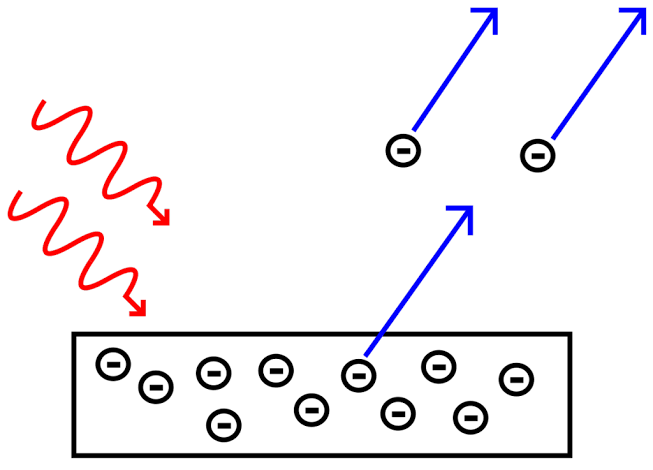
\includegraphics[width=0.5\textwidth]{figs/fotoelektrik.png}
    \caption[Interaksi fotoelektrik]{Interaksi fotoelektrik \cite{quizlet2021quantum}}
    \label{fig:photoelectric}
\end{figure}

Efek fotolistrik terjadi saat seluruh energi foton diserap oleh elektron kulit atom sehingga elektron terlepas dari atom sebagai fotoelektron \cite{jho2023discussion}. Peluang terjadinya interaksi ini meningkat pada material dengan nomor atom tinggi (\textit{high Z}) dan pada energi foton yang rendah \cite{fitri2023correlation}. Oleh karena itu, efek fotolistrik mendominasi interaksi sinar-X diagnostik maupun sinar gamma dengan energi yang 
rendah\cite{fitri2023correlation}. Setelah elektron keluar dari atom, kulit elektron akan kosong sehingga akan diisi oleh elektron dengan tingkat energi yang lebih tinggi sehingga menghasilkan sinar-X atau elektron Auger \cite{jho2023discussion}.

\begin{figure}[htbp]
    \centering
    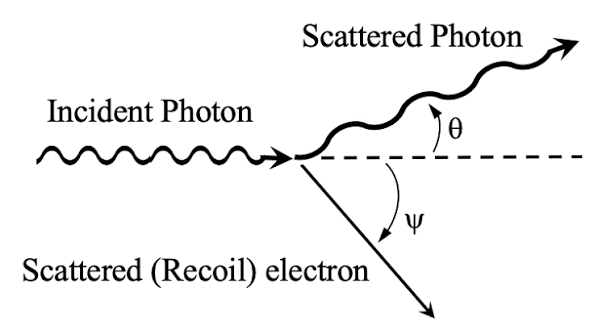
\includegraphics[width=0.5\textwidth]{figs/compton_scattering.png}
    \caption[Interaksi hamburan Compton]{Interaksi hamburan Compton \cite{monteiro2020compton}}
    \label{fig:scattering}
\end{figure}

Pada energi menengah, khususnya pada rentang energi ratusan KeV seperti sinar gamma Cs-137 sebesar 662 KeV, interaksi yang paling sering terjadi adalah interaksi hamburan Compton (\textit{Compton scattering})\cite{kierans2022compton}. Dalam proses interaksi ini, foton berinteraksi dengan elektron bebas atau elektron dengan ikatan lemah pada atom \cite{kierans2022compton}. Sebagian energi dari foton ditransfer ke elektron sehingga elektron terpental sebagai 
elektron Compton, sedangkan sisa energi dari foton tetap bergerak namun dengan energi yang lebih rendah dan arah yang berubah sesuai dari sudut hamburan ($\theta$) \cite{nguyen2011scattered}. Energi dari hamburan Compton dapat dinyatakan dengan menggunakan persamaan compton \cite{kierans2022compton}.

\begin{equation}
    E' = \frac{E}{1 + \frac{E}{m_e c^2}(1 - \cos\theta)}
\end{equation}

Dengan $E$ merupakan energi foton datang, $E'$ energi foton terhambur, $m_e c^2$ energi diam dari elektron sebesar 511 KeV, dan $\theta$ adalah sudut hamburan. Hubungan tersebut menunjukkan bahwa semakin besar sudut dari hamburannya maka energi foton yang terhambur juga akan semakin kecil. Prinsip inilah yang digunakan menjadi dasar metode Gamma Compton \textit{Backscatter} karena foton yang terpantul 
kembali menuju detektor dengan membawa informasi mengenai densitas ataupun adanya cacat dalam struktur material.

\begin{figure}[htbp]
    \centering
    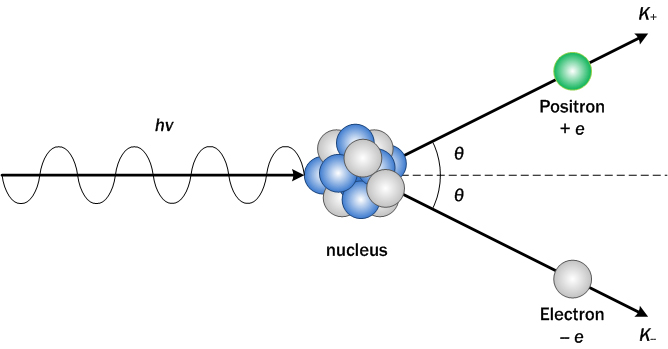
\includegraphics[width=0.8\textwidth]{figs/pair production.jpg}
    \caption[Interaksi pasangan produksi]{Interaksi pasangan produksi \cite{dasilva2012producao}}
    \label{fig:pair_production}
\end{figure}

Apabila energi foton melebihi 1,022 MeV, interaksi yang dapat terjadi adalah produksi pasangan (\textit{pair production}) \cite{kierans2022compton}. Pada mekanisme interaksi ini energi foton diubah menjadi pasangan elektron dan positron disekitar medan inti atom \cite{donner2025comparative}. Karena memerlukan energi yang minimal sebesar dua kali energi diam elektron, yaitu 1,022 MeV, maka proses ini tidak dapat terjadi pada sumber radiasi isotop Cs-137 yang hanya memiliki
energi sekitar 662 KeV \cite{marshall2025comprehensive}. Dengan demikian, penelitian ini menggunakan sumber radio isotop Cs-137, mekanisme interaksi yang paling dominan terjadi adalah hamburan Compton, mekanisme interaksi lain dapat diabaikan \cite{donner2025comparative}.

Selain mengalami hamburan, intensitas dari sinar gamma juga akan mengalami penurunan ketika melewati suatu material \cite{kierans2022compton}. Hal ini dikarenakan proses penyerapan dan hamburan yang dikenal sebagai atenuasi. Besarnya nilai dari pelemahan intensitas atau atenuasi ini mengikuti hukum Beer-Lambert yang dinyakan sebagai 

\begin{equation}
    I = I_0 e^{-\mu x}
\end{equation}

Dengan $I_0$ adalah intensitas awal, $I$ adalah intensitas setelah melewati material, $\mu$ adalah koefisien atenuasi linier, dan $x$ merupakan ketebalan material. Nilai koefisien atenuasi bergantung pada energi foton dan jenis dari material yang berinteraksi \cite{aloraini2022design}. Sehingga nilai atenuasi tersebut dapat digunakan untuk mengindentifikasi adanya perubahan struktur atau adanya cacat seperti korosi, retak, atau lubang \cite{alanazi2024evaluating}. Perubahan ini 
yang dimanfaatkan dalam sistem deteksi keretakan pipa berbasis hamburan balik sinar gamma \cite{alanazi2024evaluating}.

Pemahaman mengenai mekanisme interaksi dari radiasi gamma dengan material merupakan dasar penting dalam tahap pengembangan sistem inspeksi tanpa merusak \cite{azmi2023gamma}. Pada energi 662 KeV dari sumber Cs-137, hamburan Compton menjadi mekanisme dominan yang terjadi sehingga sangat sesuai jika digunakan sebagai prinsip \textit{tomography} untuk mendeteksi perubahan densitas maupun mendeteksi adanya retak dalam struktur pipa \cite{olshanoski2022multi}. Oleh 
karena itu, teori interaksi radiasi dengan materi menjadi landasan utama dalam permodelan simulasi dengan \textit{software} Geant4 serta rekonstruksi citra tomografi pada penelitian ini \cite{azmi2023gamma}.

\section{Sistem Deteksi dan Spektroskopi Radiasi}

Sistem deteksi radiasi merupakan suatu rangkaian perangkat yang berfungsi untuk mendeteksi adanya radiasi dan mengubah energi dari radiasi tersebut menjadi sinyal listrik yang dapat diolah menjadi informasi baik kuantitatif maupun kualitatif \cite{susanto2024kemajuan}. Sistem ini banyak dimanfaatkan dalam berbagai bidang seperti kedokteran, industri, keamanan, dan penelitian, serta \textit{non-destructive testing}. Pada penggunaan sebagai alat inspeksi 
sinar gamma, sistem deteksi berfungsi mengukur jumlah foton yang diterima dan energi yang diterima detektor setelah mengalami interaksi dengan objek yang diamati \cite{muttaqin2026rancang}. Hasil informasi dari sistem deteksi tersebut digunakan untuk mengidentifikasi adanya perubahan struktur pada material yang dapat digunakan untuk menandakan adanya cacat pada material \cite{irwansyah2019deteksi}.

Secara umum sistem deteksi radiasi memiliki komponen utama yang terdiri dari sumber radiasi, detektor, rangkaian elektronika pengolah sinyal, sistem akuisisi data, dan perangkat lunak analisis \cite{etim_digital}. Ketika radiasi memasuki sistem detektor, energi dari radiasi diubah menjadi pulsa listrik melalui mekanisme interaksi tertentu yang bergantung pada jenis bahan detektornya \cite{djokorayono2023gamma}. Pulsa listrik itu kemudian diperkuat oleh penguat (\textit{amplifier}) dan \textit{preamplifier} 
sebelum dikonversi menjadi data digital menggunakan ADC (\textit{analog to digital converter}) \cite{etim_digital}. Kemudian data dianalisis menggunakan perangkat lunak spektroskopi sehingga diperoleh informasi mengenai energi maupaun intensitas dari radiasi yang terpancar oleh sumber yang mengenai detektor. Sistem seperti ini banyak digunakan pada aplikasi inspeksi gamma berbasis hamburan balik Compton karena mampu menghasilkan data spektrum energi secara langsung \cite{zhang2023research}.

Pada penelitian ini karena menggunakan prinsip interaksi hamburan balik Compton, detektor radiasi harus mampu membedakan hamburan dari foton yang berasal dari berbagai posisi didalam material \cite{Yu2024}. Oleh karena itu, karakteristik detektor seperti efisiensi deteksi, resolusi energi, waktu respons, dan sensitivitas sangat menentukan kualitas data yang diperoleh \cite{Yu2024_arxiv}. Jenis detektor yang sering digunakan adalah detektor sintilator Sodium Iodide yang diaktivasi Talium NaI(Tl) karena 
memiliki efisiensi deteksi yang tinggi pada sinar gamma, \textit{cost} yang rendah, serta ukuran dan dimensi kristal yang dapat dibuat lebih besar sehingga meningkatkan probabilitas adanya \textit{cross section} terhadap foton \cite{Prihtiadi2018}. Meskipun energi resolusi yang dimiliki NaI(Tl) lebih kecil dibandingkan detektor semikonduktor yang lain seperti HPGe, NaI(Tl) menjadi pilihan utama dalam berbagai aplikasi industri karena praktis dan ekonomis \cite{Yu2024}.

Spektroskopi radiasi merupakan teknik analisis yang memanfaatkan distribusi energi yang diterima detektor untuk memperoleh informasi mengenai sumber radiasi maupun material yang sedang berinteraksi \cite{channappa2025standardization}. Dalam spektroskopi gamma, setiap bahan radioaktif memiliki energi foton yang berbeda sehingga dapat diidentifikasi melalui puncak (\textit{photopeak}) pada spektrum energinya \cite{mcgregor2018materials}. Selain \textit{photopeak}, spektrum gamma juga mengandung \textit{compton continuum}, \textit{compton edge}, \textit{backscatter peak}, 
dan \textit{escape peak} yang muncul akibat berbagai mekanisme interaksi foton dengan materi atau detektor \cite{kierans2022compton}. Analisis terhadap puncak-puncak tersebut memungkinkan identifikasi radionuklida serta mengevaluasi kondisi internal material yang sedang diamati \cite{aloraini2022design}.

\begin{figure}[htbp]
    \centering
    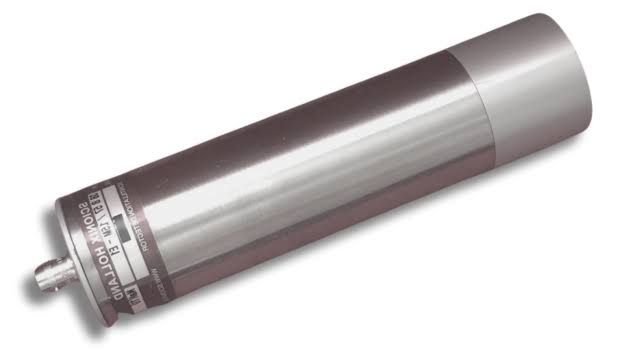
\includegraphics[width=0.8\textwidth]{figs/detektor.jpeg}
    \caption[Krista sintilator]{Kristal sintilator NaI(TI) \cite{kcsensor2026cod}}
    \label{fig:NaI(TI)}
\end{figure}

Salah satu parameter penting dalam spektroskopi gamma adalah resolusi energi (\textit{energy resolution}) yaitu kemampuan detektor dalam membedakan dua energi radiasi foton yang berdekatan nilainya \cite{demir2021determination}. Resolusi energi biasanya dinyatakan menggunakan nilai \textit{Full Width at Half Maximum} (FWHM) pada puncak dan dinyatakan dengan persamaan 
\begin{equation}
    R = \frac{FWHM}{E} \times 100\%
\end{equation}
dengan $R$ adalah resolusi energi, $FWHM$ merupakan lebar puncak pada setengah tinggi maksimum, dan $E$ adalah \textit{photopeak} \cite{ababneh2024sensitivity}. Nilai resolusi yang kecil menandakan kemampuan detektor yang baik dalam memisahkan puncak energi yang menghasilkan identifikasi bahan radioaktif yang lebih akurat \cite{demir2021determination}. Pada detektor NaI(TI), resolusi energi untuk foton Cs-137 umumnya berada pada kisaran 6-8$\%$, sedangkan pada detektor HPGe nilai resolusi 
energi berkisar pada 1\% \cite{amitasari2015pengaruh}.

\begin{figure}[htbp]
    \centering
    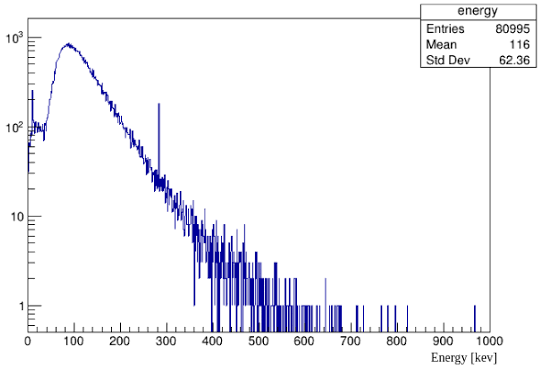
\includegraphics[width=1.0\textwidth]{figs/images (1).png}
    \caption[Spektrum energi dari Cesium-137]{Spektrum energi dari Cesium-137 \cite{geant4forum2021cs137}}
    \label{fig:energy_spectrum}
\end{figure}

Selain resolusi energi, efisiensi deteksi juga merupakan parameter penting dalam sistem spektroskopi \cite{sihotang2025analisis}. Efisiensi deteksi menunjukkan kemampuan dalam menangkap foton yang datang dan dipengaruhi oleh dimensi kristal, geometri dari sistem deteksi, energi foton, serta jarak dari sumber dengan detektor \cite{oktajianto2015gamma}. Dalam sistem detektor yang menggunakan prinsip hamburan balik Compton, efisiensi yang tinggi sangat diperlukan agar jumlah hamburan baliknya yang sedikit masih dapat direkam sehingga 
meningkatkan kualitas citra rekonstruksi \textit{tomography}. Oleh sebab itu, optimasi posisi sumber dan detektor menjadi aspek yang penting dalam penelitian berbasis simulasi \cite{oktajianto2015gamma}.

Secara keseluruhan, sistem deteksi dan spektroskopi radiasi memiliki peran yang penting dalam pengembangan teknologi inspeksi berbasis hamburan balik sinar gamma. Kemampuan sistem dalam mendeteksi perubahan energi dan jumlah hamburan menjadi dasar utama untuk memperoleh informasi struktur internal material. Pada penelitian ini, data spektrum sinar gamma yang dihasilkan oleh detektor NaI(TI) digunakan sebagai \textit{input} dalam proses analisis distribusi intensitas hamburan serta 
rekonstruksi citra tomografi guna mengidentifikasi adanya cacat pada material.

\section{\textit{Non Destructive Testing} (NDT) Pada Pipa}

\textit{Non-destructive testing} (NDT) merupakan sekumpulan metode inspeksi yang digunakan untuk mengevaluasi kondisi struktur internal suatu material, komponen, maupun struktur tanpa menyebabkan kerusakan pada objek yang sedang diamati \cite{silva2023review}. Berbeda dengan metode \textit{destructive testing} yang mengharuskan spesimen mengalami kerusakan saat proses inspeksi, metode NDT memungkinkan objek tetap dapat digunakan pasca inspeksi \cite{abdollahi2025non}. Karena itu, NDT banyak diterapkan pada beberapa industri salah 
satu contohnya adalah industri minyak dan gas (migas) \cite{wang2024basic}. Penerapan NDT bertujuan untuk mendeteksi cacat, retak, korosi, penipisan dinding pada pipa migas, maupun ketidaksempurnaan lainya sejak dini sehingga dapat mencegah kegagalan sistem perpipaan yang berpotensi merugikan banyak hal \cite{tian2024non}.

Pada industri migas, pipa merupakan komponen yang utama dalam distribusi fluida bertekanan tinggi \cite{wang2024basic}. Selama masa operasi, pipa sering kali mengalami degradasi atau penurunan kualitas akibat dari korosi internal, korosi eksternal, erosi, kelelahan material (\textit{fatigue}), maupun retak akibat tegangan (\textit{stress corossion cracking}) \cite{odor2024advanced}. Kerusakan tersebut menyebabkan berkurangnya lapisan ketebalan dinding pipa sehingga meningkatkan terjadinya kebocoran maupun kegagalan struktur \cite{tian2024non}. Oleh karena itu, 
inspeksi dengan menggunakan NDT menjadi penting dalam menjaga kualitas pipa serta memperpanjang umur pakai dari pipa tersebut \cite{silva2023review}.

Berbagai metode NDT telah banyak dikembangkan untuk mendeteksi kerusakan pada pipa dengan karakteristik material dan jenis kerusakan yang ingin diamati \cite{wang2024basic}. Metode yang umum dipakai dalam NDT antara lain visual \textit{testing} (VT), \textit{ultrasonic testing} (UT), \textit{magnetic particle testing} (MT), \textit{liquid penetrant testing} (PT), \textit{Eddy current testing} (ECT), serta \textit{radiographic testing} (RT) \cite{Huang2024}. Visual \textit{testing} digunakan pada inspeksi awal untuk melihat kondisi permukaan 
luar pipa, sedangkan \textit{ultasonic testing} memanfaat gelombang ultrasonik untuk mendeteksi cacat internal dan mengukur ketebalan dari material pipa tersebut. \textit{Magnetic particle testing} diterapkan pada material dengan sifat feromagnetik untuk mendeteksi retakan pada permukaan luar pipa, sementara \textit{liquid penetrant testing} digunakan pada material tanpa poros untuk mengidentifikasi cacat terbuka pada permukaan pipa. \textit{Eddy current testing} sering dimanfaatkan pada material konduktif 
untuk mendeteksi adanya retakan dangkal, sedangkan \textit{radiographic testing} menggunakan sinar-X maupun sinar gamma untuk memperoleh informasi kondisi internal material pipa \cite{may2022recent}.

Di antara metode tersebut, \textit{Radiographic testing} mempunyai kelebihan karena mampu memberikan informasi mengenai kondisi internal dalam pipa tanpa perlu kontak langsung dengan material pipa \cite{licata2020depicting}. Metode ini memanfaatkan radiasi pengion berupa sinar-X atau sinar gamma yang dilewatkan melalui material \cite{silva2023review}. Perbedaan intensitas yang ditangkap oleh detektor setelah melakukan interaksi dengan material digunakan untuk menggambarkan perubahan densitas maupun keberadaan cacat di dalam objek. Teknik radiografi biasa umumnya 
membutuhkan akses pada kedua sisi pipa, yaitu satu sisi sumber dan sisi lainya adalah bagian detektor \cite{licata2020depicting}. Kondisi ini menjadi hambatan pada sistem inspeksi perpipaan yang telah terpasang di lapangan karena dalam beberapa kasus pipa yang dapat diakses hanya satu sisi saja .

Untuk mengatasi batasan tersebut, dikembangkan metode Gamma Compton \textit{Backscatter} yang memanfaatkan foton hamburan Compton sebagai sumber informasi \cite{licata2020depicting}. Berbeda dengan radiografi transmisi, metode ini menempatkan sumber radiasi dan detektor pada sisi yang sama dari objek sehingga inspeksi dapat dilakukan meskipun akses hanya tersedia pada satu sisi permukaan pipa saja \cite{licata2020depicting}. Ketika foton gamma memasuki material, sebagian foton mengalami hamburan Compton dan dipantulkan kembali menuju ke detektor \cite{margret2018scales}. Intensitas foton
hamburan dipengaruhi oleh densitas atau kepadatan elektron material sehingga perubahan akibat adanya cacat dalam dinding pipa dapat diidentifikasi melalui perubahan nilai jumlah cacahan foton yang diterima detektor \cite{margret2018scales}.

Perkembangan teknologi komputasi juga mendorong pemanfaatan simulasi monte carlo dalam pengembangan sistem inpeksi tanpa merusak (NDT) berbasis radiasi \cite{qin2023study}. Simulasi menggunakan \textit{software} Geant4 memungkinkan peneliti mensimulasikan interaksi radiasi dengan material secara akurat sehingga berbagai konfigurasi sumber, detektor, energi gamma, serta geometri objek dapat dianalisis tanpa harus melakukan eksperimen fisik yang memiliki \textit{cost} tinggi \cite{agostinelli2003geant4}. Selain itu, hasil dari simulasi dapat digunakan untuk 
mengoptimasi posisi detektor, jumlah detektor, sudut hamburan, serta parameter akuisisi data guna meningkatan sensitivitas sistem dalam mendeteksi cacat yang berukuran orde mikroskopis \cite{qin2023study}.

Pada penelitian ini menggunakan metode gamma compton \textit{backscatter} sebagai teknik inspeksi \textit{non-destruktif} untuk mendeteksi cacat pada pipa migas. Sistem inspeksi dimodelkan dengan Geant4 dengan sumber radiasi gamma Cesium-137 dan detektor NaI(TI). Informasi atau hasil output simulasi berupa distribusi jumlah foton hamburan kemudian dianalisis menggunakan metode rekonstruksi citra tomografi untuk menggambarkan posisi dan ukuran keretakan di dalam pipa. Pendekatan ini diharapkan mampu menghasilkan 
sistem inspeksi yang efektif, aman, dan dapat diaplikasikan pada kondisi lapangan memiliki keterbatasan akses terhadap objek.

\section{Pemodelan Transportasi Partikel dengan Monte Carlo Geant4}

Metode Monte Carlo merupakan suatu metode komputasional numerik berbasis probabilitas yang menggunakan bilangan acak (\textit{random number}) untuk menyelesaikan masalah matematis dan fisika yang sulit diselesaikan secara analitik \cite{agma2025simulasi}. Metode ini pertama kali dikembangkan pada akhir tahun 1940-an dalam proyek \textit{Manhattan} untuk memodelkan transportasi neutron dan hingga saat ini menjadi salah satu pendekatan utama dalam simulasi interaksi radiasi dengan materi \cite{sood2021neutronics}. Prinsip dasar metode monte carlo adalah melakukan 
simulasi terhadap sejumlah besar riwayat (\textit{particle histories}) dari setiap individu partikel sehingga karakteristik statistik dari seluruh partikel dapat digunakan untuk memperkirakan besaran yang diinginkan \cite{agma2025simulasi}. Semakin banyak jumlah perulangan simulasinya (\textit{number of histories}), maka nilai ketidakpastian hasil simulasi akan menjadi lebih kecil sehingga akurasi akan meningkat \cite{agma2025simulasi}.

Dalam simulasi monte carlo, lintasan partikel ditentukan oleh probabilitas adanya terjadi interaksi dengan material yang dilewatinya \cite{agma2025simulasi}. Besarnya peluang suatu partikel mengalami interaksi bergantung pada nilai koefisen atenuasi linier ($\mu$) yang berkaitan dengan penampang lintang interaksi (\textit{cross section}) \cite{agma2025simulasi}. Hubungan antara koefisien atenuasi dan panjang lintasan rata-rata (\textit{mean free path}) dinyatakan dengan persamaan berikut
\begin{equation}
    \lambda = \frac{1}{\mu}
\end{equation}
dengan $\lambda$ adalah panjang lintasan bebas rata - rata (cm), dan $\mu$ merupakan koefisien atenuasi linier ($cm^-1$). Persamaan tersebut menunjukkan semakin besar nilai dari koefisien atenuasi linier, maka semakin pendek jarak yang ditempuh partikel sebelum mengenai material untuk berinteraksi \cite{agma2025simulasi}.

Pada metode monte carlo, jarak tempuh partikel menuju interaksi berikutnya tidak ditentukan secara tetap, melainkan didapatkan dari hasil menggunakan bilangan acak yang mengikuti distribusi eksponensial \cite{yusmaity2019simulasi}. Panjang lintasan partikel dihitung dengan persamaan :
\begin{equation}
    s = -\lambda ln (\xi)
\end{equation}
dengan $s$ merupakan panjang lintasan partikel sebelum mengalami interaksi, sedangkan $\xi$ adalah bilangan acak yang terdistribusi seragam pada rentang $ 0 < \xi < 1$ \cite{agma2025simulasi}. Persamaan ini menjadi dasar algoritma pengacakan (\textit{particle tracking}) pada hampir seluruh \textit{software} simulasi monte carlo, termasuk Geant4 \cite{agostinelli2003geant4}.

Selama proses transportasi partikel, setiap foton yang terpancar akan mengalami berbagai kemungkinan terjadinya interaksi sesuai dengan probabilitas yang ditentukan oleh penampang lintang material \cite{agma2025simulasi}. Kemungkinan tersebut dihitung berdasarkan total penampang lintang yang merupakan penjumlahan dari seluruh proses interaksi yang mungkin terjadi \cite{agma2025simulasi}.
\begin{equation}
    \sigma_{total} = \sigma_{pe} + \sigma_{c} + \sigma_{pp}
\end{equation}
dengan $\sigma_{pc}$ merupakan penampang lintang efek fotolistrik(\textit{photoelectric effect}), $\sigma_c$ adalah penampang lintang dari hamburan Compton (\textit{Compton scattering}),sedangkan $\sigma_{pp}$ merupakan penampang lintang dari interaksi pasangan produksi (\textit{pair production}). Pada rentang energi sebesar 662 KeV yang dipancarkan 
oleh radio isotop Cesium-137, mekanisme interaksi yang sering terjadi adalah hamburan Compton dibanding dengan dua mekanisme interaksi lainnya sehingga cocok digunakan pada penelitian ini.

Transportasi partikel merupakan proses pemodelan dari lintasan partikel saat bergerak melewati suatu materi sambil mengalami perubahan energi, arah dari gerak, maupun pembentukan partikel kedua akibat dari interaksi \cite{alghamdi2022geant4}. Pada setiap langkah (\textit{tracking step}), algoritma dari monte carlo menentukan secara \textit{random} jenis dari interaksi yang akan 
dialami suatu partikel berdasarkan data penampang lintang yang tersedia di \textit{physics list} \cite{agma2025simulasi}.Setelah terjadi suatu interaksi, energi partikel, arah gerak, serta kemungkinan terbentuknya partikel sekunder akan dihitung kembali hingga partikel kehilangan seluruh energinya, keluar dari geometri sistem maupun mengalami absorpsi \cite{agma2025simulasi}.

Keunggulan dari metode monte carlo ini dibanding dengan pendekatan analitis terletak pada kemampuannya dalam memodelkan geometri yang kompleks dan berbagai proses fisika secara bersamaan. Dalam bidang fisika radiasi, metode ini banyak digunakan untuk memodelkan simulasi dosimetri, pencitraan medis, proteksi radiasi, desain detektor, radiografi industri, 
serta inspeksi non destruktif. Selain menghasilkan estimasi distribusi flux partikel, monte carlo juga mampu menghitung deposisi energi, efisiensi detektor, probabilitas hamburan, hingga distribusi dosis dengan tingkat akurasi yang tinggi.

Salah satu \textit{software} monte carlo yang banyak digunakan dalam penelitian fisika energi tinggi dan fisika partikel adalah Geant4 (\textit{Geometri and Tracking}). Geant4 merupakan \textit{software open-source} yang dikembangkan oleh tim kolaborasi internasional CERN untuk mensimulasikan transportasi dari suatu partikel melalui materi. Perangkat lunak ini 
menyediakan banyak modul dan \textit{package} untuk mendefinisikan geometri tiga dimensi, material, sumber partikel, proses fisika elektromagnetik maupun hadronik, sistem pelacakan partikel (\textit{tracking}) serta pencatatan hasil simulasi (\textit{scoring}).

Pada Geant4, simulasi dimulai dengan mendefinisikan geometri sistem, material penyusun, posisi sumber radiasi, dan konfigurasi detektor \cite{agma2025simulasi}. Kemudian menentukan penggunaan \textit{physics list} yang sesuai dengan rentang energi partikel \cite{rizani2012simulasi}. Setelah partikel primer ditembakkan, Geant4 melakukan pelacakan (\textit{tracking}) seluruh lintasan dari partikel beserta partikel 
sekunder yang dihasilkan akibat dari mekanisme interaksi yang terjadi \cite{agma2025simulasi}. Seluruh informasi dari hasil simulasi dapat direkam sebagai \textit{output} simulasi untuk dianalisis lebih lanjut.

\begin{figure}[htbp]
    \centering
    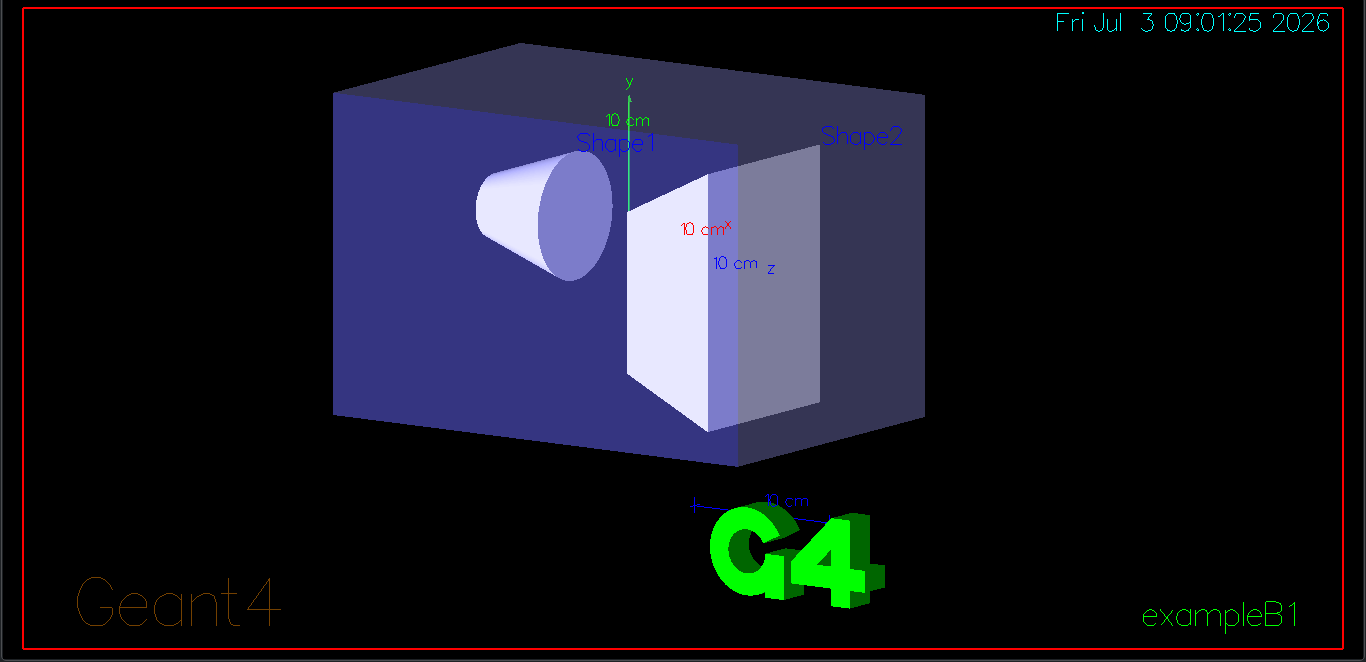
\includegraphics[width=0.8\textwidth]{figs/geant4.png}
    \caption{Tampilan geometri Geant4}
    \label{fig:Geant4}
\end{figure}

Pada penelitian ini metode monte carlo digunakan untuk memodelkan sistem detektor keretakan pipa dengan menggunakan prinsip interaksi hamburan balik Compton menggunakan sumber radiasi Cesium-137 dan detektor NaI(TI). Simulasi dilakukan dengan Geant4 untuk memodelkan transport partikel foton gamma dari sumber menuju ke material target yaitu pipa, proses hamburan 
Compton, hingga foton hamburan diterima oleh detektor. Data hasil simulasi berupa jumlah cacahan foton dan distribusi energi hamburan yang kemudian digunakan sebagai \textit{input} dalam proses rekonstruksi citra tomografi untuk melihat bentuk dan ukuran dari keretakan yang ada di dalam pipa.

% ==========================================
% BAB 3 METODOLOGI PENELITIAN
% ==========================================
\chapter{METODE PENELITIAN}

\section{Rancangan Penelitian}
Penelitian ini dirancang sebagai studi ekspimen kompuatasional kuantitatif untuk mengevaluasi secara sistematis sensitivitas dari metode hamburan balik 
Compton untuk mendeteksi adanya anomali berupa keretakan (\textit{crack}) pada suatu sistem perpipaan. Rancangan penelitian ini menggunakan \textit{framework} 
simulasi monte carlo dengan menggunakan \textit{software} Geant4, dimana simulasi fisika (penembakan dan pelacakan partikel foton dari sumber Cesium-137) dijalankan 
sepenuhnya di dalam lingkungan simulasi Geant4. Kemudian, setelah dilakukan simulasi data hasil pelacakan dieksekusi menggunakan skrip analisis komputasi yaitu CERN ROOT++ 
\textit{Framework Analysis} yang berbasis C.

\begin{figure}[htbp]
  \begin{adjustwidth}{-1.5cm}{-1.5cm} % Melebarkan margin kiri dan kanan sebesar 1.5 cm
    \centering
    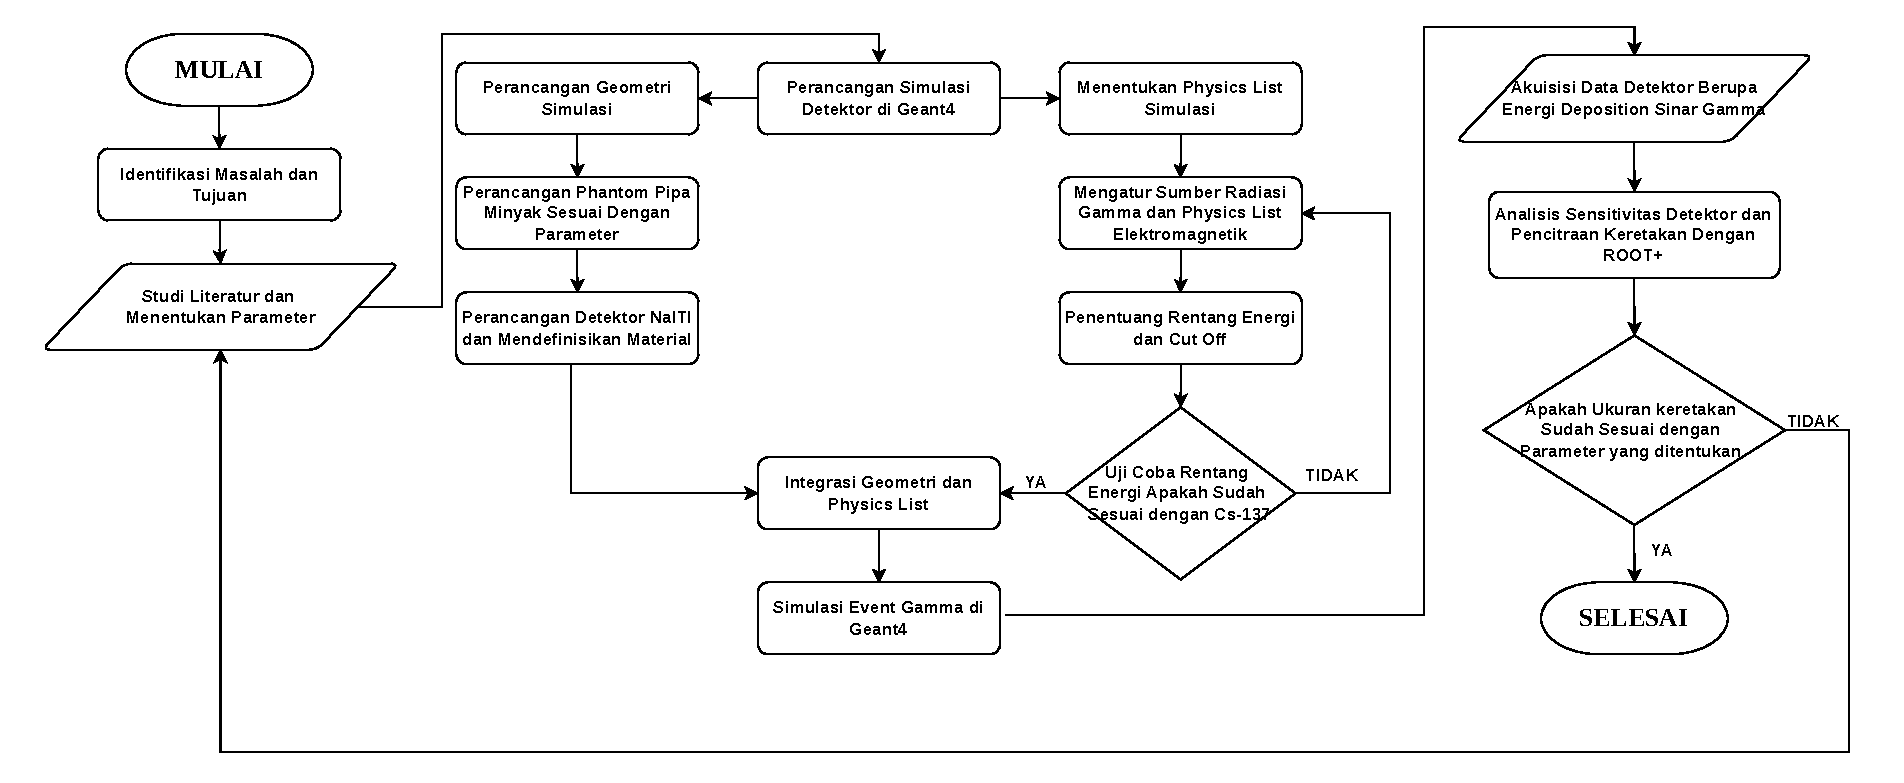
\includegraphics[width=\linewidth]{figs/flowchat.pdf}
    \caption{Diagram alir penelitian}
    \label{fig:diagram_alir}
  \end{adjustwidth}
\end{figure}

\section{Tempat dan Waktu Penelitian}
\subsection{Tempat Penelitian}
sebagian besar eksperimen komputasional dan analisis data dilakukan dengan memanfaatkan fasilitas komputasi dari \textit{High Performance Computer} (HPC) milik kelompok keahlian bidang 
(KBK) Fisika Komputasi dan Teoriti, Departemen Fisika, Universitas Negeri Malang.


\subsection{Waktu Penelitian}
Penelitian ini dilaksanakan dalam waktu kurun 6 Bulan, dimulai dari bulan Agustus 2026 hingga Januari 2027.
\begin{table}[H]
\centering
\caption{Jadwal kegiatan penelitian}
\label{tab:jadwal-penelitian}
\begin{tabular}{|c|>{\raggedright\arraybackslash}p{6cm}|c|c|c|c|c|c|}
\hline
\textbf{No} & \textbf{Kegiatan} & \textbf{Agu} & \textbf{Sep} & \textbf{Okt} & \textbf{Nov} & \textbf{Des} & \textbf{Jan} \\
\hline
1 & Studi literatur dan pemahaman roadmap Geant4 & \cellcolor{lightgreen} & \cellcolor{lightgreen} &  &  &  &\\
\hline
2 & Pemodelan geometri keretakan pipa dan detektor NaI(Tl) &  & \cellcolor{lightgreen} & \cellcolor{lightgreen} &  &  &\\
\hline
3 & Eksekusi simulasi Monte Carlo &  &  & \cellcolor{lightgreen} & \cellcolor{lightgreen} &  &\\
\hline
4 & Pengolahan data spektrum energi dengan script ROOT/C++ &  &  &  & \cellcolor{lightgreen} &  &\\
\hline
5 & Analisis spektrum dan fitting Gaussian &  &  &  & \cellcolor{lightgreen} & \cellcolor{lightgreen} &\\
\hline
6 & Evaluasi sensitivitas detektor dan analisis hasil &  &  &  &  & \cellcolor{lightgreen} &\\
\hline
7 & Penulisan proposal, laporan akhir, dan publikasi &  &  &  &  & & \cellcolor{lightgreen} \\
\hline
\end{tabular}
\end{table}


\section{Prosedur Penelitian}
\subsection{Variabel Penelitian}
\begin{itemize}
    \item Variabel Bebas    : Ukuran keretekan, bentuk keretakan
    \item variabel Terikat  : Spektrum energi hamburan balik, jumlah cacahan, fluk gamma, Nilai perbedaan relatif, citra tomografi
    \item Variabel Kontrol  : Jumlah detektor, sumber radiasi (Cesium-137), geometri simulasi.
\end{itemize}


\subsection{\textit{Benchmarking} Simulasi Geant4}
Tahap awal penelitian dilakukan dengan melakukan proses \textit{bernchmarking} simulasi untuk memvalidasi model simulasi Geant4 dan merepresentasikan respon detektor terhadap
sumber radiasi gamma sebelum digunakan pada simulasi dengan konfigurasi penuh. Prose validasi ini memiliki tuuan agar model simulasi mampu menghasilkan spektrum energi yang memiliki 
karkateristik yang sesuai dengan hasil pengukuran eksperimen sehingga model yang dibangun dapat digunakan sebagai gambaran sistem nyata. \textit{Benchmarking} dilakukan dengan sumber 
radioaktif Cesium-137 yang merupakan sumber radiasi gamma standart yang banyak digunakan dalam kalibarasi spektrometer gamma.

Pada tahap ini dibangun model simulasi menggunakan \textit{software} Geant4 dengan mendefinisikan seluruh komponen geometri sistem deteksi yang digunakan pada proses \textit{benchmarking}, meliputi 
sumber radiasi, detektor, dan kolimator. material penyusun setiap komponen didefinisikan berdasarkan \textit{database NIST MATERIAL DATABASE} yang tersedia didalam Geant4 sehingga sifat dari 
material yang mengalami interaksi dengan foton dapat direpresentasikan secara realistis. Proses dari transportasi partikel dihitung menggunakan \textit{physics list} elektromagnetik yang mencakup 
interaksi hamburan Compton, efek fotolistrik, dan produksi pasangan, yang sesuai dengan rentang energi Cs-137.

\begin{figure}[htbp]
    \centering
    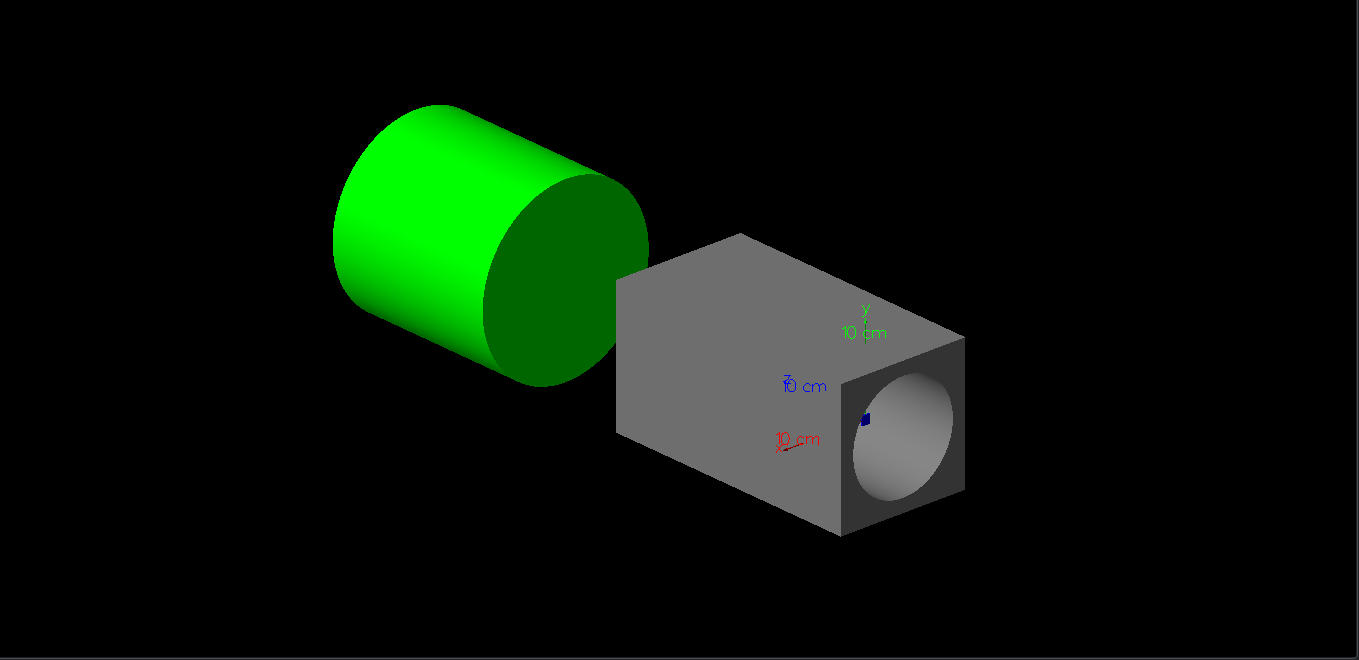
\includegraphics[width=0.8\textwidth]{figs/benchmark.png}
    \caption{Geometri \textit{benchmarking} Cesium-137}
    \label{fig:benchmarking}
\end{figure}

Secara statistik, nilai eror dari hasil simulasi monte carlo mengkuti distribusi Poisson sehingga standart deviasi jumlah cacahan yang diberikan oleh 
\begin{equation}
    \sigma N = \sqrt{N}
\end{equation}
dengan $N$ adalah jumlah cacahan yang diterima dari setiap \textit{channel}. Ketidakpastian relatif dari simulasi dapat dihitung dengan menggunakan persamaan
\begin{equation}
    \delta = \frac{\sigma N}{N} \times 100\% = \frac{1}{\sqrt{N}} \times 100\%
\end{equation}
Persamaan tersebut menunjukkan bahwa peningkatan jumlah partikel primer akan menurunkan eror hasil simulasi. Oleh karena itu, jumlah partikel primer yang digunakan 
saat proses \textit{benchmarking} dipilih cukup besar agar nilai eror dapat diminimalkan.

Spektrum yang dihasilkan oleh Geant4 masih berupa spektrum yang ideal karena belum mempertimbangkan adanya batasan resolusi energi. Oleh karena itu dilakukan proses 
\textit{Gaussian Smearing} untuk mensimulasikan pelebaran \textit{peak} yang terjadi pada sistem deteksi nyata.

Distribusi Gaussian yang digunakan pada proses \textit{smearing} dijelaskan dengan persamaan 
\begin{equation}
    G(E) = \frac{1}{\sigma \sqrt{2\pi}} exp[-\frac{(E - E_0)^2}{2\sigma^2}]
\end{equation}
dengan $E_0$ merupakan energi hasil simulasi Geant4, $E$ adalah energi setelah proses \textit{smearing}, dan $\sigma$ adalah standart deviasi dari distribusi Gaussian.

Secara numerik, energi hasil \textit{smearing} diperoleh dengan menambahkan bilangan acak yang mengikuti prinsip distribusi normal ke setiap energi hasil simulasi
\begin{equation}
    E_{smear} = E + \sigma Z
\end{equation}
dengan $E_{smear}$ adalah energi setelah dilakukan proses \textit{gaussian smearing}, $E$ merupakan energi hasil simulasi Geant4, $\sigma$ adalah standart deviasi dari 
distribusi gaussian, sedangkan $Z$ merupakan bilangan yang acak yang mengikuti distribusi normal standart $N(0,1)$. Persamaan ini digunakan pada proses setelah pemrosesan untuk 
menghasilkan spektrum energi yang mendekati respon detektor NaI(TI) pada kondisi eksperimen.

Nilai simpangan baku diperoleh dari hubungan antara nilai \textit{Full Width at Half Maximum} (FWHM) dan resolusi energi pada detektor,
\begin{equation}
    FWHM = 2.355\sigma
\end{equation}
sedangkan untuk resolusi energi dapat menggunakan persamaan
\begin{equation}
    R = \frac{FWHM}{E} \times 100\%
\end{equation}
Dengan R merupakan resolusi energi detektor pada energi $E$. Pada penelitian ini, nilai resolusi energi diperoleh melalui proses kalibrasi detektor menggunakan sumber gamma dan 
digunakan sebagai parameter utama pada proses \textit{Gaussian Smearing}.

\subsection{Implementasi Geometri Pipa dan Detektor NaI(Tl)}
Setelah model simulasi divalidasi, tahap selanjutnya adalah membangun geometri simulasi sistem deteksi keretakan dengan menggunakan \textit{software} Geant4. Implementasi dilakukan untuk 
membuat bentuk konfigurasi dari sistem inspeksi berbasis Gamma Compton \textit{Backscatter}, yang terdiri dari pipa, sumber radiasi gamma Cesium-137, dan detektor NaI(TI). Model diharapkan mampu 
menggambarkan kondisi inspeksi secara nyata sehingga proses transportasi partikel dapat disimulasikan secara akurat.

Objek yang disimulaskan berupa silinder berongga dengan menggunakan kelas \textit{G4Tubs}, dengan parameter berupa jari-jari dalam, jari-jari luar, serta panjang dari pipa. Material penyusun pipa 
didefinisikan berdasarkan komposisi material pipa migas dengan menggunakan \textit{database} material NIST yang ada pada Geant4. Untuk membuat kondisi retak beberapa simulasi ditambahkan dengan ukuran dan 
posisi keretakan tertentu.

Sumber gamma yang digunakan adalah radionuklida Cesium-137 yang memancarkan energi sebesar $661,657 KeV$. Posisi sumber berada diluar pipa dengan orientasi tegak lurus terhadap permukaan pipa sehingga 
foton dapat dipancarkan dan berinteraksi dengan pipa menghasilkan hamburan. Konfigurasi ini dipilih karena dapat mendeteksi adanya hamburan balik karena detektor dan sumber ada di sisi yang sama.

Sistem detektor terdiri atas enam buah detektor NaI(TI) yang disusun secara melingkar (mengelilingi sumber radiasi) yang ditunjukkan oleh Gambar \ref{fig:geometri_pipa}. Setiap detektor dimodelkan sebagai silinder menggunakan 
kelas \textit{G4Tubs} dan ditempatkan pada jarak tetap terhadap sumber radiasi dengan orientasi menghadap ke permukaan pipa. Konfgurasi ini untuk menangkap sudut deteksi hamburan balik. Sehingga probabilitas foton hamburan 
mencapai volume sensitif detektor dapat dimaksimalkan.
\begin{figure}[htbp]
    \centering
    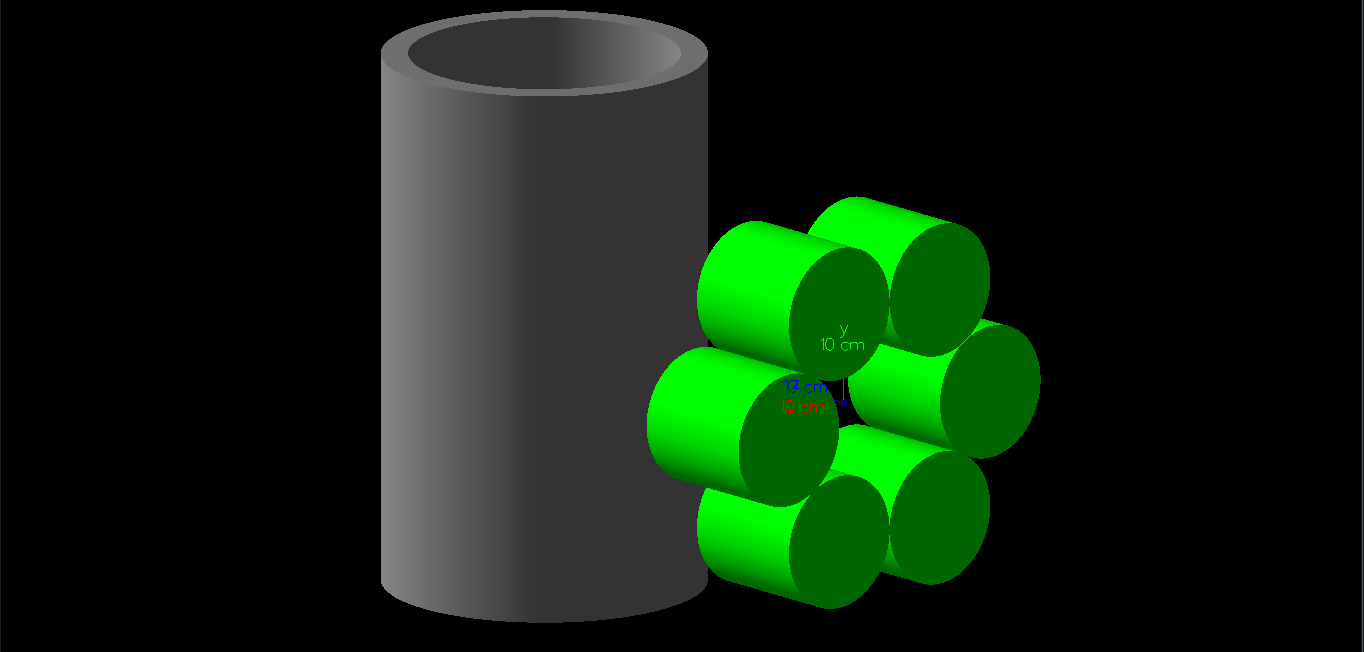
\includegraphics[width=0.8\textwidth]{figs/geometri_pipa_simulasi.png}
    \caption{Geometri simulasi sistem deteksi keretakan pipa}
    \label{fig:geometri_pipa}
\end{figure}

Selama proses simulasi, foton gamma yang dpancarkan oleh Cesium-137 ditransportasikan melalu material pipa dengan model fisika elektromagnetik pada Geant4. Pada rentang energi 662 KeV interaksi yang dominan terjadi adalah hamburan compton 
mengikuti persamaan 
\begin{equation}
    E' = \frac{E}{1 + \frac{E}{m_e c^2}(1 - \cos\theta)}
\end{equation}
dengan $E$ adalah energi foton datang, $E'$ energi foton terhambur, $m_e c^2$ energi diam dari elektron sebesar 511 KeV, dan $\theta$ adalah sudut hamburan. Foton yang mengalami hamburan Compton akan dipantulkan kembali menuju detektor sehingga 
dapat diukur jumlah cacahannya. Perubahan jumlah cacahan yang diterima detektor digunakan untuk mengidentifikasi adanya perubahan densitas akibat keretakan pada pipa.

Energi yang terdeposit pada volume sensitif direkam menggunakan mekanisme \textit{Sensitive Detector} pada Geant4. Total energi deposisi dihitung sebagai 
\begin{equation}
    E_{dep} = \sum_{i=1}^{n} \Delta E_i
\end{equation}
dengan $E_{dep}$ adalah total energi yang terdeteksi oleh detekor dan $\Delta E_i$ adalah energi yang ditransfer pada setiap proses interaksi. Selain energi deposisi, jumlah foton yang terdeteksi juga akan dicatat untuk setiap detektor dan dinyatakan sebagai 
\begin{equation}
    N = \sum_{i=1}^{n} 1
\end{equation}
dengan $N$ merupakan jumlah foton yang dterima oleh volume sensitif.

\subsection{Implementasi Sistem Pemindaian}
Setelah geometri sistem berhasil diimplementasikan, tahap berikutnya adalah membuat sistem pemindaian (\textit{scanning}) untuk memperoleh data hamburan pada setiap posisi pengukuran. Pada penelitian ini, objek pipa dibuat tetap (\textit{fixed geometry}), sedangkan 
sumber radiasi Cs-137 dan enam detektor NaI(TI) yang bergerak secara bersamaan sebaga satu modul pada sepanjang area inspeksi. Konfigurasi tersebut menerapkan prinsip \textit{Gamma Compton Backsactter}, sehingga seluruh pemindaian dilakukan hanya dari satu sisi pipa saja.

Pemindaian dilakukan dengan menggunakan koordinat kartesian dengan membagi area inspeksi menjadi banyak titik pengamatan (\textit{scan points}). Posisi sumber dan detektor pada setiap titik dinyatakan dengan persamaan \
\begin{equation}
    P_i = (x_i, y_i)
\end{equation}
Dengan $x_i$ dan $y_i$ merupakan koordinat titik pemindauan ke-i. Jumlah keseluruhan titik pemindaian dihitung menggunakan
\begin{equation}
    N_s = N_x \times N_y
\end{equation}
dengan $N_p$ merupakan jumlah partikel primer pada setiap titik pemindaian 

Selama proses simulasi berlangsung, setiap detektor merekam deposisi energi serta jumlah cacahan foton hamburan yang diterima oleh detektor sensitif. informasi tersebut kemudian disimpan sebagai \textit{output} simulasi yang berisi, koordinat pemindaian, \textit{detector id}, jumlah 
partikel primer, deposisi energi dan jumlah cacahan foton untuk setiap titik pengukuran.

Data hasil pemindaian dari seluruh titik selanjutnya digabung menjadi satu basis data (\textit{dataset}) yang digunakan sebagai \textit{input} pada tahap evaluasi dan analisi. Dataset tersebut menjadi dasar dari proses normalisasi, perhitungan parameter, rekonstruksi untuk mengidentifikasi adanya 
keretakan pada pipa

\subsection{Evaluasi dan Analisis data}
Data hasil simulasi Geant4 berupa koordinat titik pemindaian, identitas detektor, jumlah partikel primer, energi deposisi, dan jumlah cacahan pada setiap detekor terlebih dahulu dijadikan satu dataset untuk memudahkan proses analisis. Seluruh proses pengolahan data dilakukan dengan menggunakan 
\textit{software} ROOT CERN sehingga diperoleh parameter kuantitatif yang digunakan untuk mengevaluasi respon sistem deteksi terhadap keberadaan keretakan pada pipa.

Tahap awal analisis dilakukan melalui normalisasi jumlah cacahan terhadap jumlah partikel primer untuk menghilangkan pengaruh variasi statistik selama proses simulasi. Nilai cacahan yang dinormalikan dapat dihitung dengan menggunakan
\begin{equation}
    C_{norm} = \frac{N_{count}}{N_p}
\end{equation}
dengan $C_{norm}$ adalah cacahan ternormalisasi, $N_{count}$ adalah jumlah foton yang terdeteksi, dan $N_P$ merupakan jumlah partikel primer pada setiap posisi pemindaian.

Perubahan respon sistem deteksi akibat adanya keretakan dievaluasi menggunakan metode \textit{Relative Difference} (RD) dengan membandingkan kondisi pipa utuh dan pipa yang ada retak. Nilai \textit{Relative Difference} dihitung menggunakan
\begin{equation}
    RD = \frac{C_{crack} - C_{normal}}{C_{normal}}
\end{equation}
dengan $C_{crack}$ merupakan cacahan ternormalisasi pada kondisi pipa retak dan $C_{normal}$ merupakan cacahan ternormalisasi pada kondisi pipa utuh. Distribusi nilai RD digunakan sebagai parameter utama untuk melihat perubahan intensitas hamburan yang disebabkan oleh adanya keretakan pada pipa

Karena data hasil pemindaian diperoleh dalam bentuk titik-titik diskrit, hasil tersebut perlu diolah dengan interpolasi spasial untuk membentuk distribusi data kontinu pada bidang yang diamati. Selanjutnya menerapkan Gaussian filter untuk mengurangi fluktuasi statistik akibat adanya eror pada simulasi Monte Carlo 
tanpa menghilangkan karakteristik citra utama
\begin{equation}
    G(x,y) = \frac{1}{2\pi\sigma^2} exp(- \frac{x^2 + y^2}{2\sigma^2})
\end{equation}
dengan $\sigma$ merupakan simpangan baku distribusi Gaussian yang mengontrol tingkat penghalusan citra

Citra tomografi kemudian direkonstruksi menggunakan metode \textit{backprojection}, yaitu dengan menjumlahkan kontribusi nilai \textit{Relative Difference} dari seluruh posisi \textit{scanning} terhadap piksel citra. intensitas dari rekonstruksi dinyatakan sebagai
\begin{equation}
    I(x,y) = \sum_{i = 1}^{N} RD_i W_i (x,y)
\end{equation}
dengan $I(x,y)$ merupakan intensitas piksel pada koordinat (x,y), $RD_i$ adalah nilai \textit{Relative Difference} pada titik pemindaian ke-i, sedangkan $W_i(x,y)$ merupakan fungsi pembobot yang menggambarkan kontribusi dari masing - masing titik pemindaian terhadap piksel citra.

Hasil rekonstruksi kemudian dievaluasi berdasarkan distribusi dari intensitas untuk mengidentifikasi dimana lokasi keretakan muncul. Posisi keretakan ditentukan melalui adanya intensitas maksimum (\textit{hotspot}) yang dirumuskan sebagai 
\begin{equation}
    I_{max} = max[I(x,y)]
\end{equation}
sedangkan kualitas rekonstruksi dievaluasi menggunakan RMSE (\textit{root mean square error})
\begin{equation}
    RMSE = \sqrt{\frac{1}{n} \sum_{i = 1}^{n}(y_i - \hat{y_i}^2)}
\end{equation}
dengan $y_i$ merupakan data referensi atau normal dan $\hat{y_i}$ merupakan hasil rekonstruksi pada titik ke-i. Nilai RMSE berfungsi untuk mengevaluasi tingkat kesesuaian hasil rekonstruksi terhadap kondisi normal

Seluruh parameter hasil analisi berupa distribusi \textit{relative difference}, citra hasil \textit{backprojection}, lokasi \textit{hostpot}, dan nilai RMSE dgunakan untuk mengevaluasi hasil dari sistem detektor hamburan balik sinar gamma 
dalam mendeteksi keretakan didalam struktur internal pipa.

% ==========================================
% DAFTAR PUSTAKA
% ==========================================
\renewcommand{\bibname}{DAFTAR PUSTAKA}
\bibliographystyle{unsrt} % Style agar referensi urut [1], [2], dst sesuai kemunculan di teks
\bibliography{ref}   % Memanggil file cas-refs.bib yang kita buat tadi

\end{document}